\section{Method}
\subsection{Time-stamped Transcript}
Several on-line video lectures (e.g. Khan Academy) come with transcripts. In cases where transcripts were not provided, we used an on-line audio transcription service to acquire a verbatim text transcript. Then, we used a tool from \cite{rubin2013content} to compute an alignment between the video's audio file and the transcript. The final output is a time-stamped transcript, where each word is annotated with a start and end time.

\subsection{Stroke Extraction}
A \textit{stroke} is defined as the set of foreground pixels that is drawn during one continuous drawing activity. The method used to extract strokes from video frames are similar to that used by \cite{monserrat2013notevideo} to extract visual objects in their NoteVideo interface. Figure~\ref{Fig:stroke_examples} shows examples of extracted strokes from different videos. A typical stroke comprises several characters to several words, or it can also be a part of other drawings such as a graph (Figure~\ref{Fig:stroke_examples}c).  

\begin{figure}[h]
       \centering
        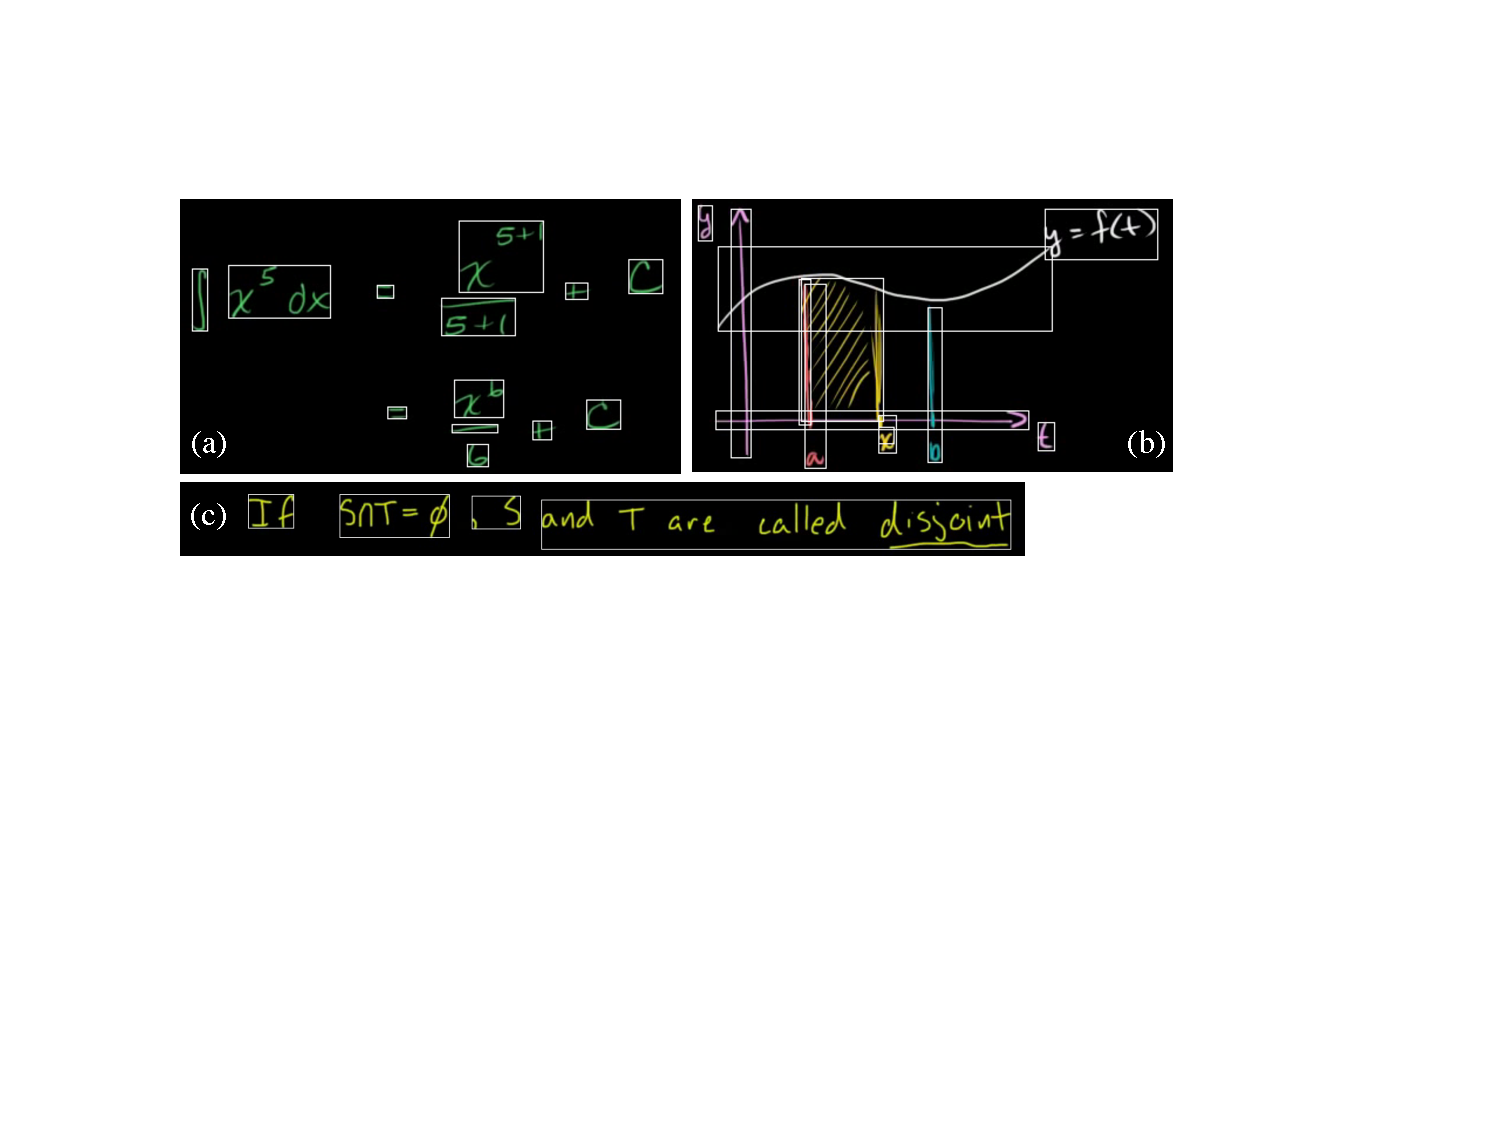
\includegraphics[width=0.45\textwidth, clip=true]{images/example_strokes}
        \caption{Examples of strokes extracted from different videos.}
        \label{Fig:stroke_examples}
\end{figure}

\subsection{Hierarchical Grouping of Strokes}
We group strokes into hierarchical units: lines and sentence-strokes.  
A line consists of a set of strokes that \textit{belong together} semantically. For example, a line could be a single row of equations, or a graph including its labels. Figure~\ref{Fig:line_examples} shows examples of lines. The problem of grouping strokes into lines is analogous to the problem of line breaking, also known as word wrapping \cite{knuth1981breaking}. An important difference is that in the traditional word wrapping problem, only a contiguous set of words can be put in the same line. In our case, strokes in a single line can be interspersed by strokes in a different line. This happens, for example, when the instructor goes back and forth between two lines of equations, or between a graph and an equation (Figures~\ref{Fig:line_order}). 

Scoring function description

Pseudo code figure
\begin{algorithm}[h]
\DontPrintSemicolon
\SetAlgoLined
\SetCommentSty{\small\ttfamily} 
  \SetKwInOut{Input}{Input}\SetKwInOut{Output}{Output}
  \Input{list of strokes ${S}$}
  \Output{list of optimal lines, ${L_{\left\vert{S}\right\vert}}$}
  $L_{-1} =$ \string{\string} \tcp{$L_i=$ optimal set of lines upto $i$-th stroke}\;
    \For{each stroke $s_i \in \mathbf{S}$}{
    \textit{minscore} = $+\infty$\;
    \For{$j \leftarrow -1$ \textbf{to} $i-1$}{
      \For{$n \leftarrow 0$ \textbf{to} $\left\vert{L_j}\right\vert+1$}{
        \tcp{score to merge $s_i$ to $n$-th line of $L_j$}\;
        \tcp{If $n = \left\vert{L_j}\right\vert+1$, $s_i$ on a new line by itself.}\;
        \textit{score} $\leftarrow$ line\_score($L_{j}$, $n$)\;
        \If {score \textless minscore}{
          ${optj} = j$\;
          ${optn} = n$\;
        }
      }
   }
   $L_i=$ merge $s_i$ to $optn$-th line of $L_{optj}$\;
}

\end{algorithm}

\begin{figure*}[h]
        \centering
        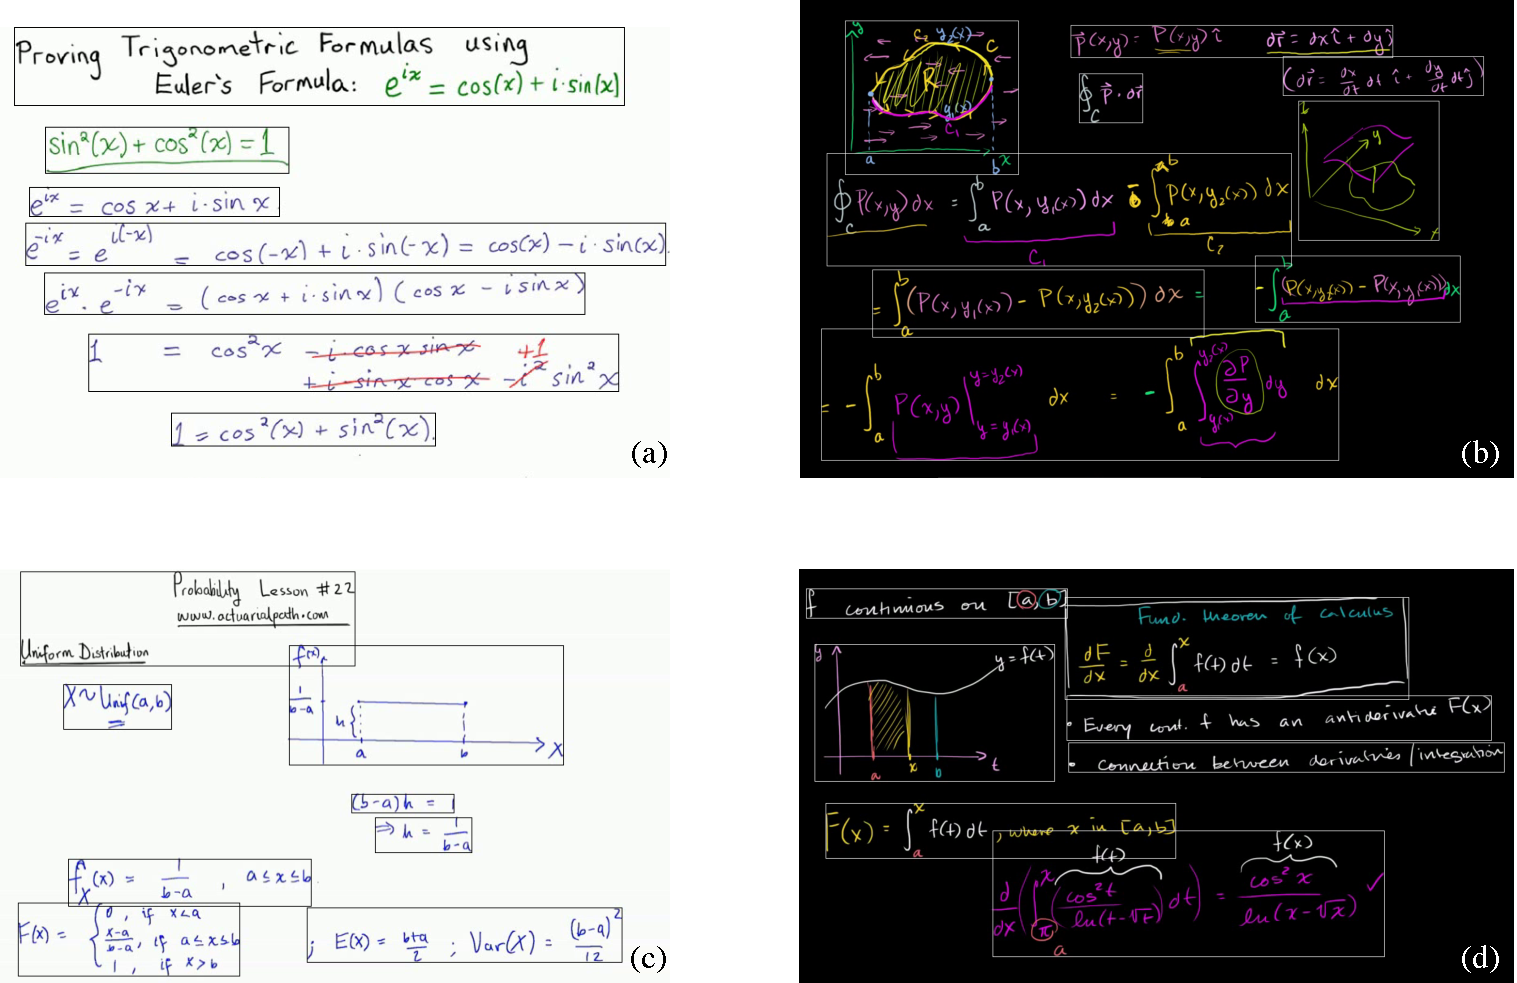
\includegraphics[width=0.9\textwidth]{images/example_lines}
        \caption{Examples of lines (i.e. set of strokes that belong together semantically) output from our line-breaking algorithm. Our algorithm successfully identifies meaningful groups even from complex layouts with a mix of equations, figures and graphs.}
        \label{Fig:line_examples}
\end{figure*}

Sentence is a meaningful unit. So, we divide the strokes in a line to sentence-strokes.

In summary, we have the following hierarchical grouping of strokes: strokes, sentence-strokes, and lines.



\subsection{Layout}


